% !TeX program = xelatex
% !TeX spellcheck = de_DE
\documentclass{beamer}
\usepackage{fontspec}
\usepackage{polyglossia}
\usepackage[notocbib]{apacite}
\usepackage{hyperref}
\usepackage{xspace}
\usepackage{array}
\usepackage{fontawesome}
\usepackage[normalem]{ulem}

% taken from http://tex.stackexchange.com/questions/45912/box-around-a-few-items-in-an-itemize-environment

\usepackage{xparse}%  For \NewDocumentCommand
\usepackage{calc}%    For the \widthof macro
\usepackage{tikz}
\usetikzlibrary{calc}

\newcommand{\tikzmark}[1]{\tikz[overlay,remember picture] \node (#1) {};}

\NewDocumentCommand{\DrawBoxWide}{s O{}}{%
    \tikz[overlay,remember picture]{
    \IfBooleanTF{#1}{%
        \coordinate (RightPoint) at ($(left |- right)+(\linewidth-\labelsep-\labelwidth,0.0)$);
    }{%
        \coordinate (RightPoint) at (right.east);
    }%
    \draw[red,#2]
      ($(left)+(-\labelwidth,0.9em)$) rectangle
      ($(RightPoint)+(0.2em,-0.3em)$);}
}

\setsansfont{Calibri}
\setdefaultlanguage{german}
\usetheme{UHH}

\def\authors#1#2{\author[#1]{#2}}
\def\email#1{\texttt{#1}}
\title{Resilient Distributed Systems}
\subtitle{Tooling aka. auf dem Weg zum „Incident Monitor”}
\authors{Felix~Ortmann}{Felix~Ortmann\\ \email{\{0ortmann\}@informatik.uni-hamburg.de}}
\institute{Universität Hamburg\\Fachbereich Informatik\\Vogt-Kölln-Straße 30\\22527 Hamburg}


\date{\today}
\titlegraphic{
\includegraphics[width=3cm]{img/uhh.pdf}}

\renewcommand{\APACrefauthstyle}{\bfseries}
\setcounter{tocdepth}{1}
\def\tocname{Gliederung des Vortrags}
\AtBeginSection{\frame{\frametitle{\tocname}\tableofcontents[currentsection]}}

\newcolumntype{x}[1]{>{\centering\arraybackslash}m{#1}}
\setbeamertemplate{headline}[default]

\defbeamertemplate*{title page}{customized}[1][]
{
	{\color{leuchtrot}
	\usebeamerfont{title}\centering\inserttitle\par
	\centering\usebeamerfont{subtitle}\insertsubtitle\par}
	\bigskip
	\centering\usebeamerfont{author}\insertauthor\par
	\bigskip
	\usebeamerfont{institute}\insertinstitute\par
	\bigskip
	\usebeamerfont{date}\insertdate\par
}
\setbeamertemplate{itemize/enumerate body begin}{\large}

\begin{document}

\fontsize{14pt}{14pt}
	
% Titelfolie
{\setbeamercolor{title page}{bg=leuchtrot}
\begin{frame}%
	\titlepage
\end{frame}}

% Gliederung
\begin{frame}{\tocname}
	\tableofcontents
\end{frame}

\section{Daten Daten Daten...}

\begin{frame}{\insertsection}
	\fontsize{20pt}{7.2}\selectfont
	„Zur Datenanalyse brauchen wir Daten. Diverse Probleme entstehen.“
\end{frame}

\begin{frame}{\insertsection}
	\begin{itemize}
		\setlength\itemsep{1em}
		\item Erhebung (andere Vorträge, Bro, OSQuery, Metrics etc)
		\item Kollektion
		\item Persistenz
		\item (zielführende) Durchsuchbarkeit gewährleisten
		\item Visualisierung ($\approx$ Querying)
	\end{itemize}
\end{frame}

\section{Daten Kollektion}

\begin{frame}{\insertsection}
	\begin{itemize}
		\setlength\itemsep{0.7em}
		\item Ziel: zentrale „Sammelstelle”
		\item Fetch: 
			\begin{itemize}
				\setlength\itemsep{1em}
				\item Aktiv: Senden an Kollektor
				\item Passiv: Crawlen von erhobenen Metriken/Daten
			\end{itemize}
		\item Process: 
			\begin{itemize}
				\setlength\itemsep{1em}
				\item Umformung von Formaten
				\item Typisierung bsp. für ES-Schema
			\end{itemize}
		\item Ship: 
			\begin{itemize}
				\setlength\itemsep{1em}
				\item Übertragung an (remote) DB
				\item Einhaltung von Schema
			\end{itemize}
	\end{itemize}
\end{frame}

\begin{frame}{\insertsection}
	Diverse Lösungen existieren, vornehmlich für Logs
	\begin{itemize}
		\item Logstash
		\item Papertrail
		\item syslog-ng
		\item fluentd
	\end{itemize}
	Oder Metric-Scraping
	\begin{itemize}
		\item Prometheus
		\item Telegraf
	\end{itemize}
	Hier (wsl) uninteressant, weil Broker!
\end{frame}


\section{Datenbanken}


\begin{frame}{\insertsection}
	\fontsize{20pt}{20pt}\selectfont
	Wahl der DB abhängig von Art der Informationen, die gespeichert werden sollen
\end{frame}


\begin{frame}{ElasticSearch}
	\begin{itemize}
		\setlength\itemsep{1em}
		\item Volltext durchsuchbar
		\item „alle Daten”
		\item Real-Time
		\item Query-Mächtigkeit gewaltig (Lucene)
		\item Dokumentenorientiert
		\item Kein Schema
		\item Verteilt \& hochverfügbar
	\end{itemize}
\end{frame}

\begin{frame}{InfluxDB}
	\begin{itemize}
		\setlength\itemsep{1em}
		\item Zeit-Serien Datenbank (Metriken)
		\item denkbar für z.B. Verbindungsdaten
		\item Real-Time
		\item Anomalie-Erkennung auf DB-Ebene
		\item Verteilt \& hochverfügbar
	\end{itemize}
\end{frame}

\section{Visualisierungstools}

\begin{frame}{\insertsection\ -- Kibana}
	\begin{itemize}
		\item aufsetzend auf ES
		\item ES-Query Visualisierung
		\item Haupt-Usecase: Analyse, etwa Korrelation von Logs
	\end{itemize}
	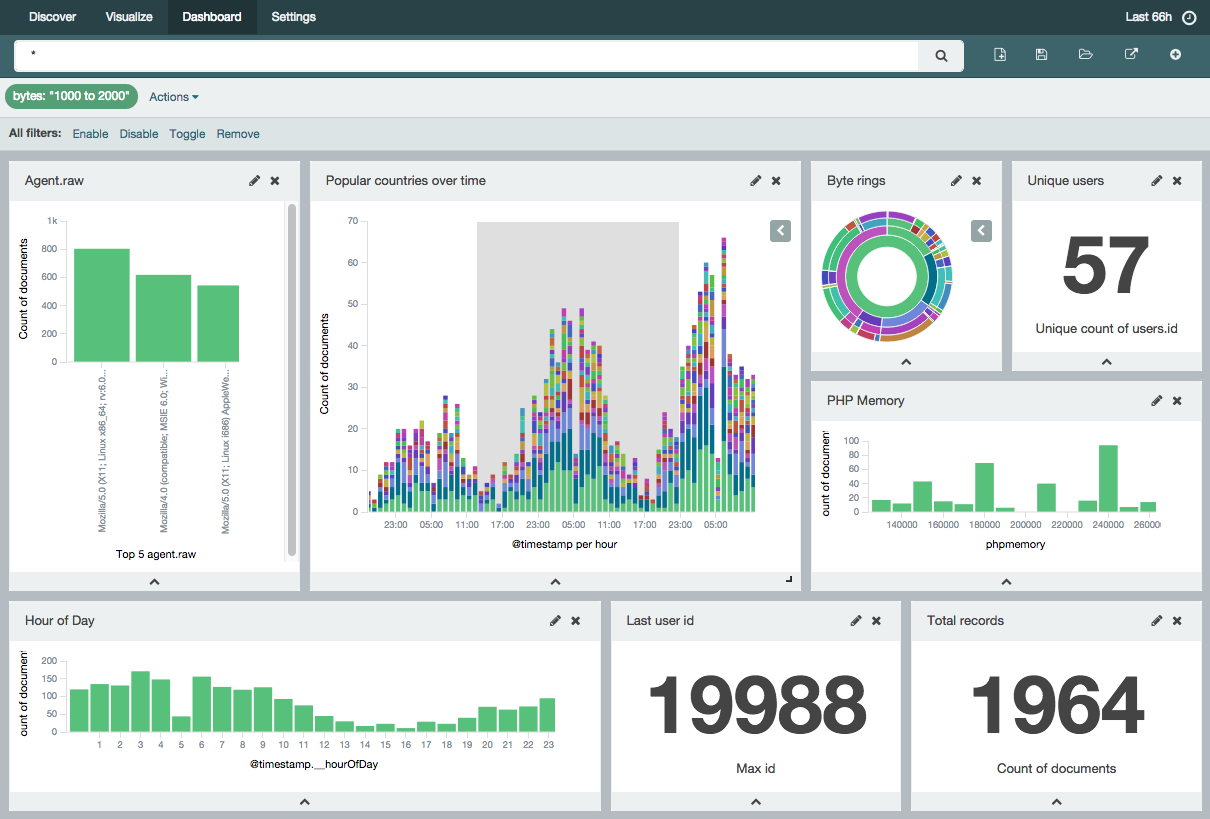
\includegraphics[width=\linewidth,page=1]{img/kibana.png}
\end{frame}

\begin{frame}{\insertsection\ -- Grafana}
	\begin{itemize}
		\item auf ES, InfluxDB, Graphite etc...
		\item Zeit-Serien-Metrik Visualisierung
		\item Visualisierung, nicht Analyse!
	\end{itemize}
	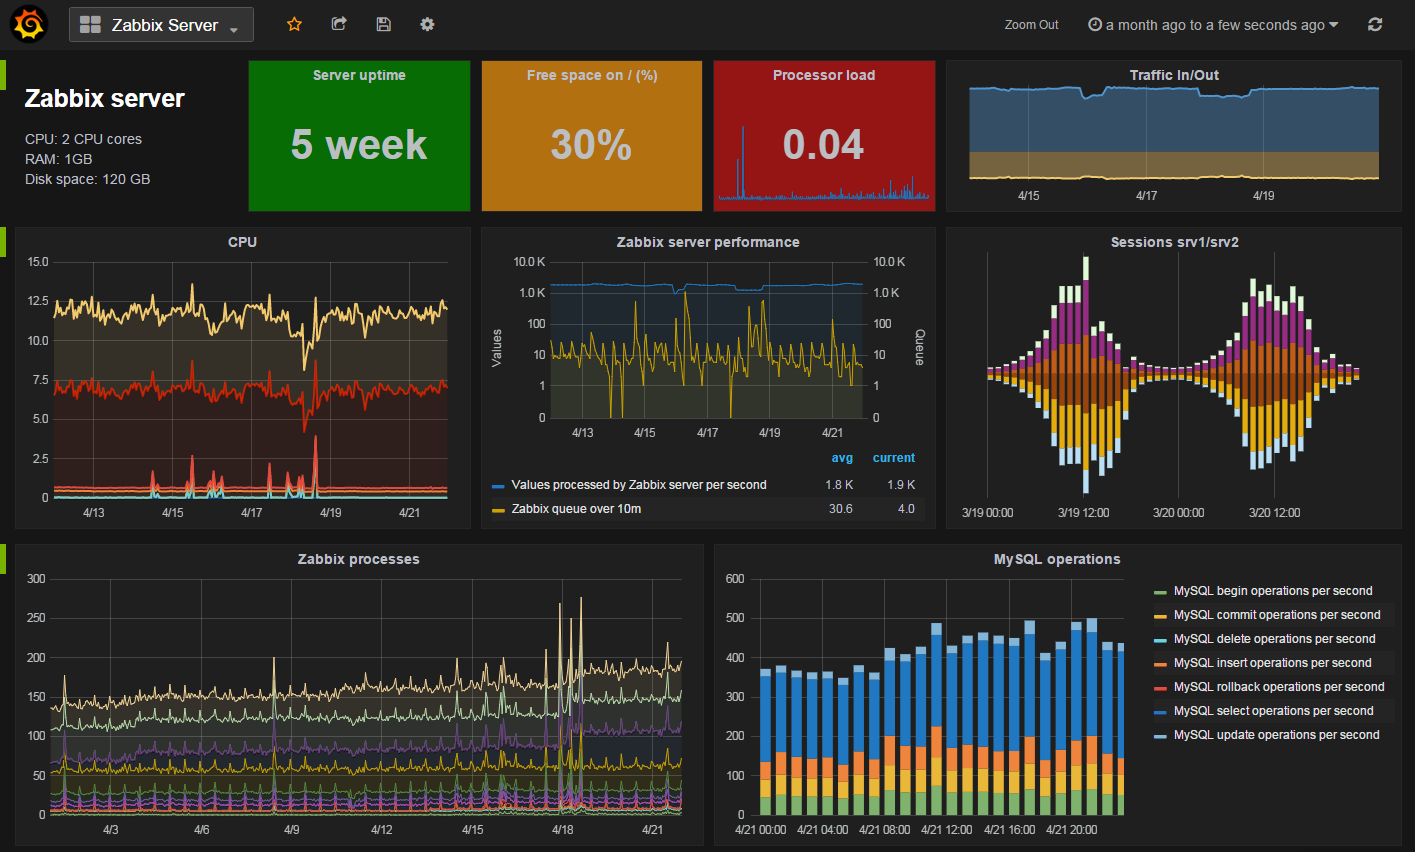
\includegraphics[width=\linewidth,page=1]{img/grafana.png}
\end{frame}

\begin{frame}{\insertsection\ -- Chronograf}
	\begin{itemize}
		\item Wie Grafana zur Zeit-Serien-Metrik Visualisierung
		\item Etwas neuer / netter im Umgang als Grafana
		\item super integriert mit InfluxDB, da gleicher Hersteller
	\end{itemize}
	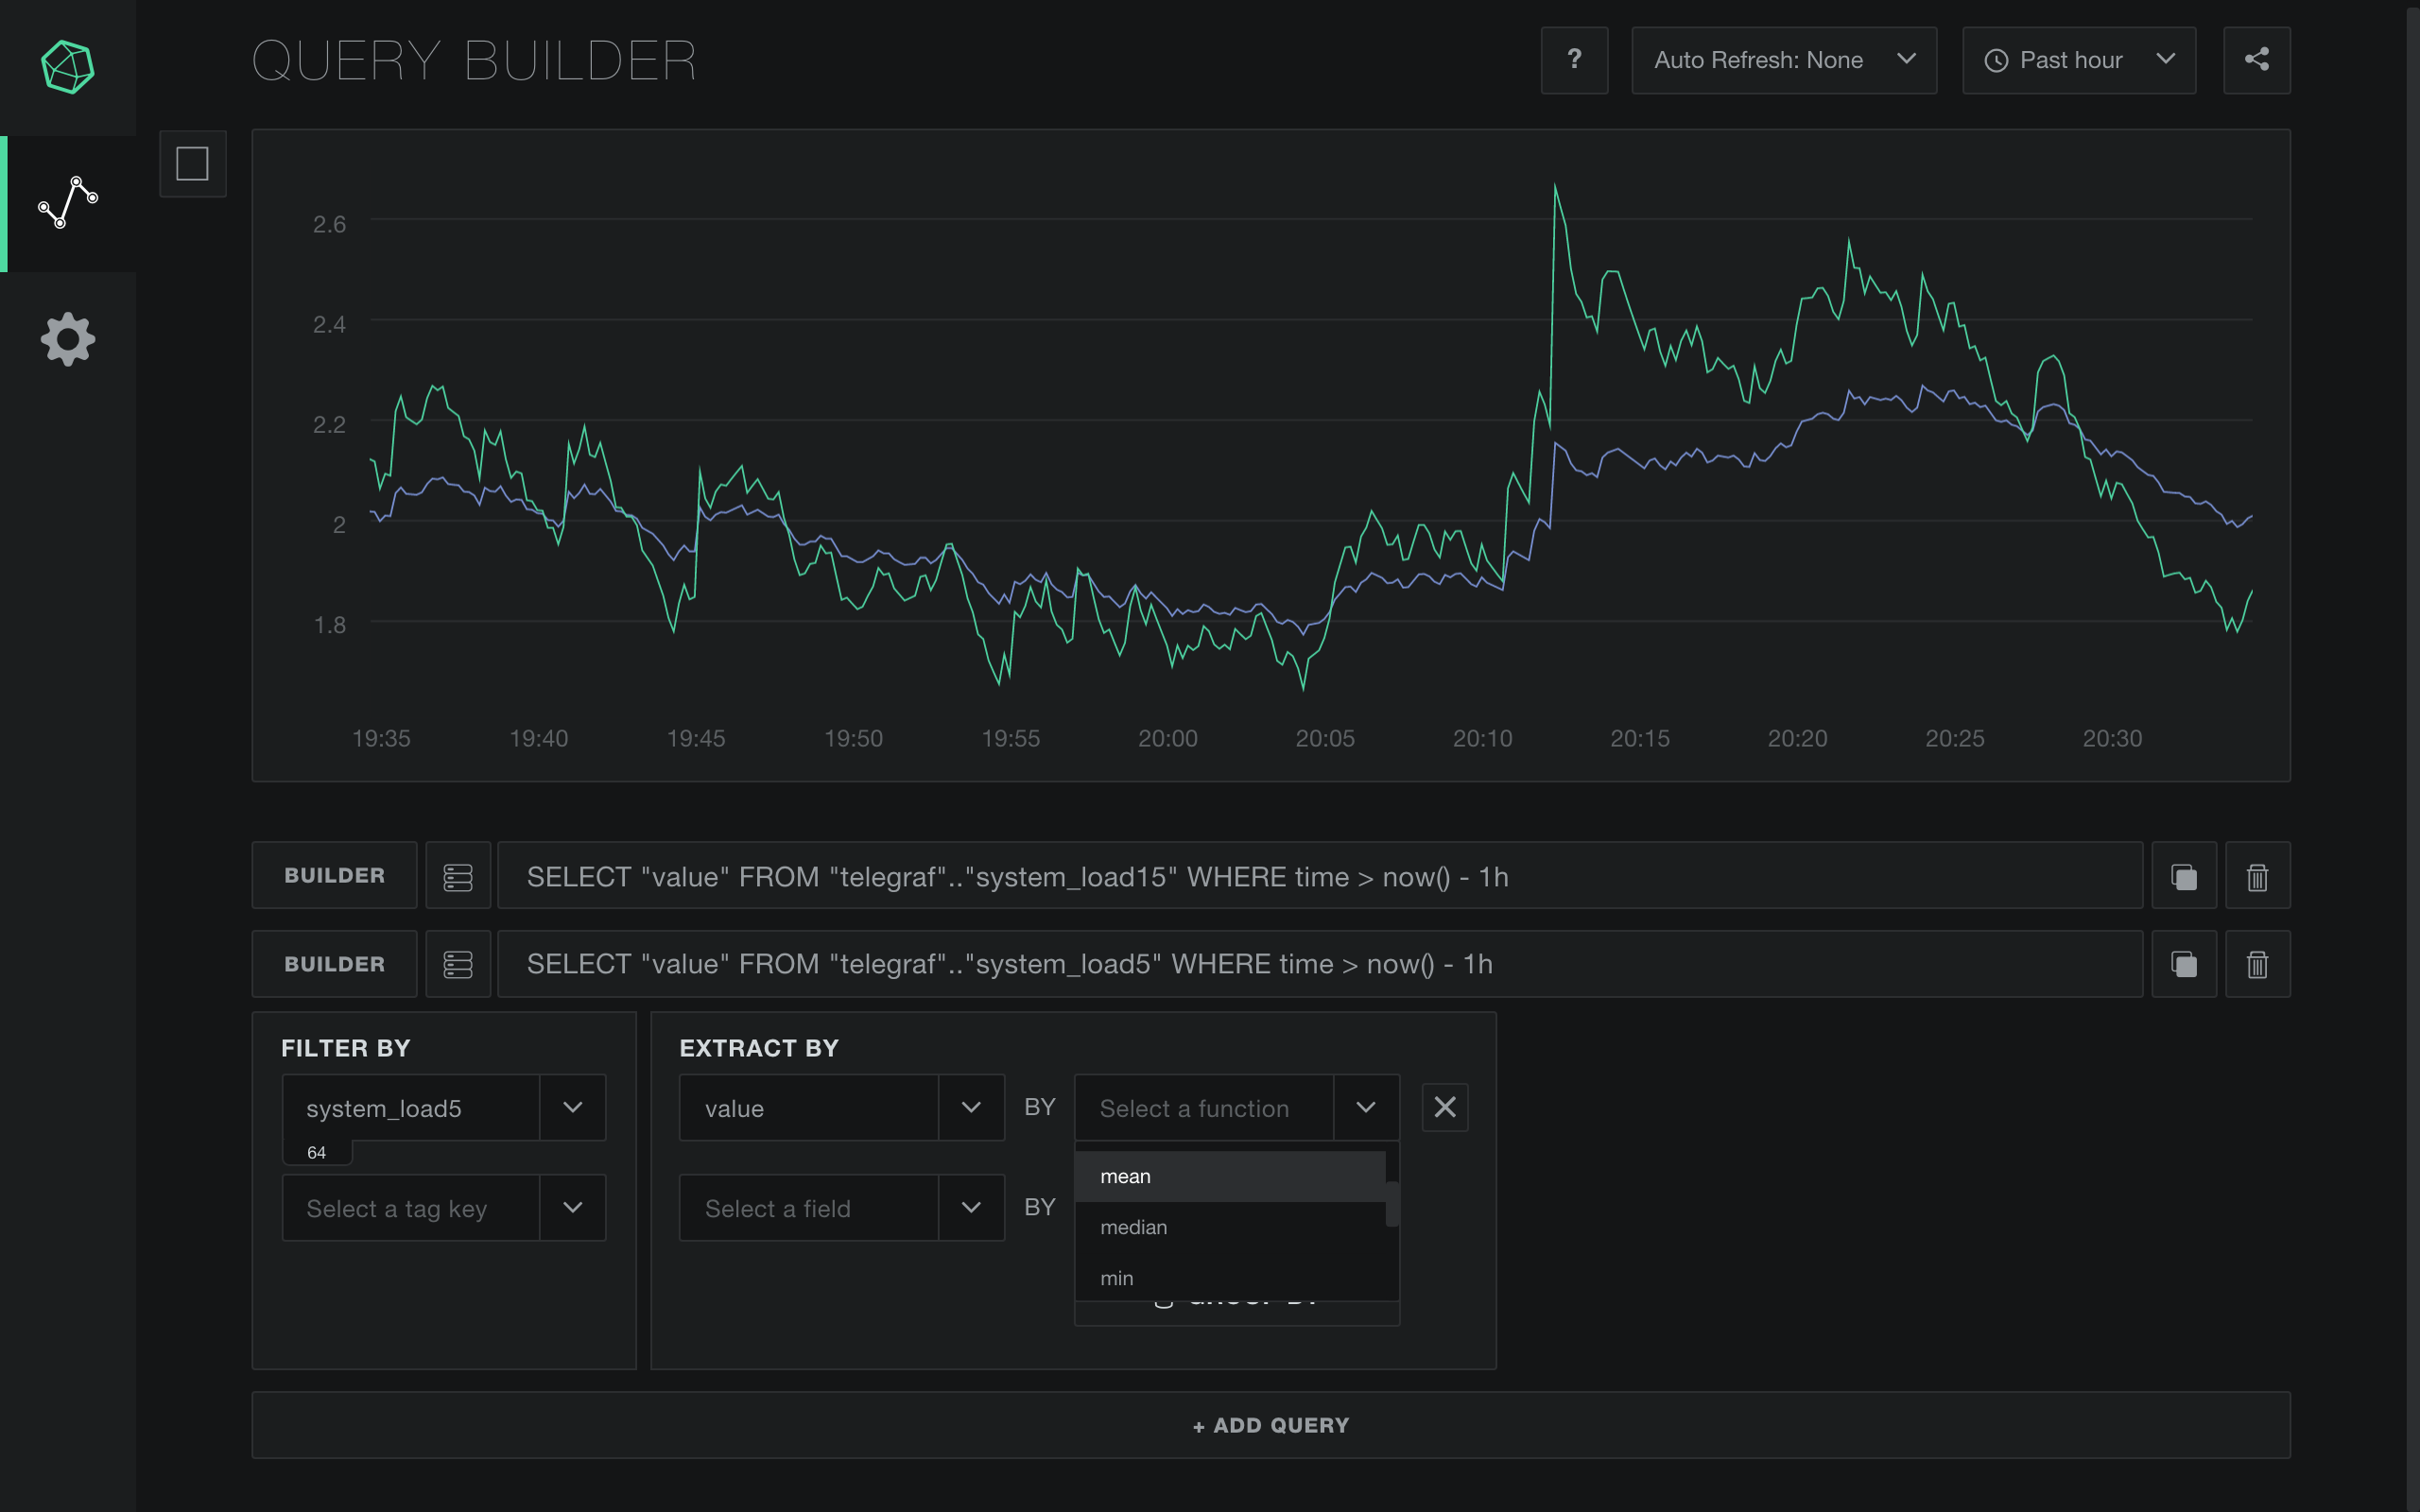
\includegraphics[width=0.8\linewidth,page=1]{img/chronograf.png}
\end{frame}

\section{Stacks}

\begin{frame}{\insertsection\ -- ELK}
	\underline{ELK:} Elasticsearch -- Logstash -- Kibana
	Volltextdurchsuchbarkeit -- Logprocessing \& Shipping -- Query Visualisierung
	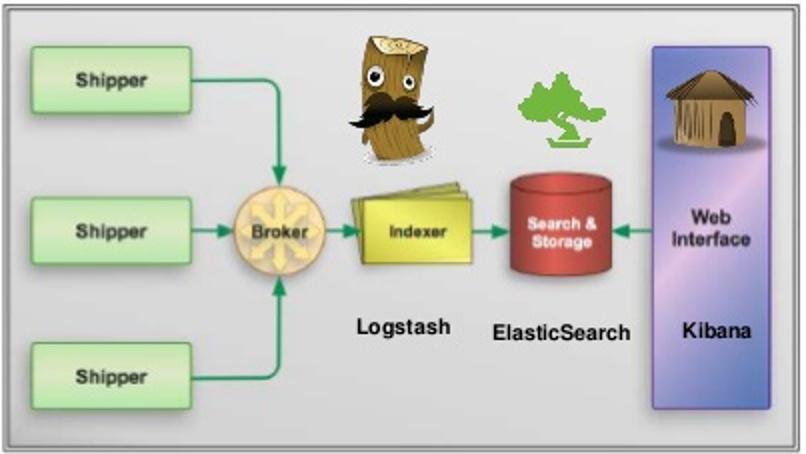
\includegraphics[width=0.8\linewidth,page=1]{img/ELK-stack.jpg}\\
	\fontsize{4pt}{7.2}\selectfont
	\textit{http://www.slideshare.net/GlobalLogicUkraine/the-elk-stack-get-to-know-logs-igor-rudyk}
\end{frame}

\begin{frame}{\insertsection\ -- TICK}
	\underline{TICK:} Telegraf -- InfluxDB -- Chronograf -- Kapacitor\\
	Metrik-Erhebung -- Time-Series-Database -- Visualisierung -- Alerting
	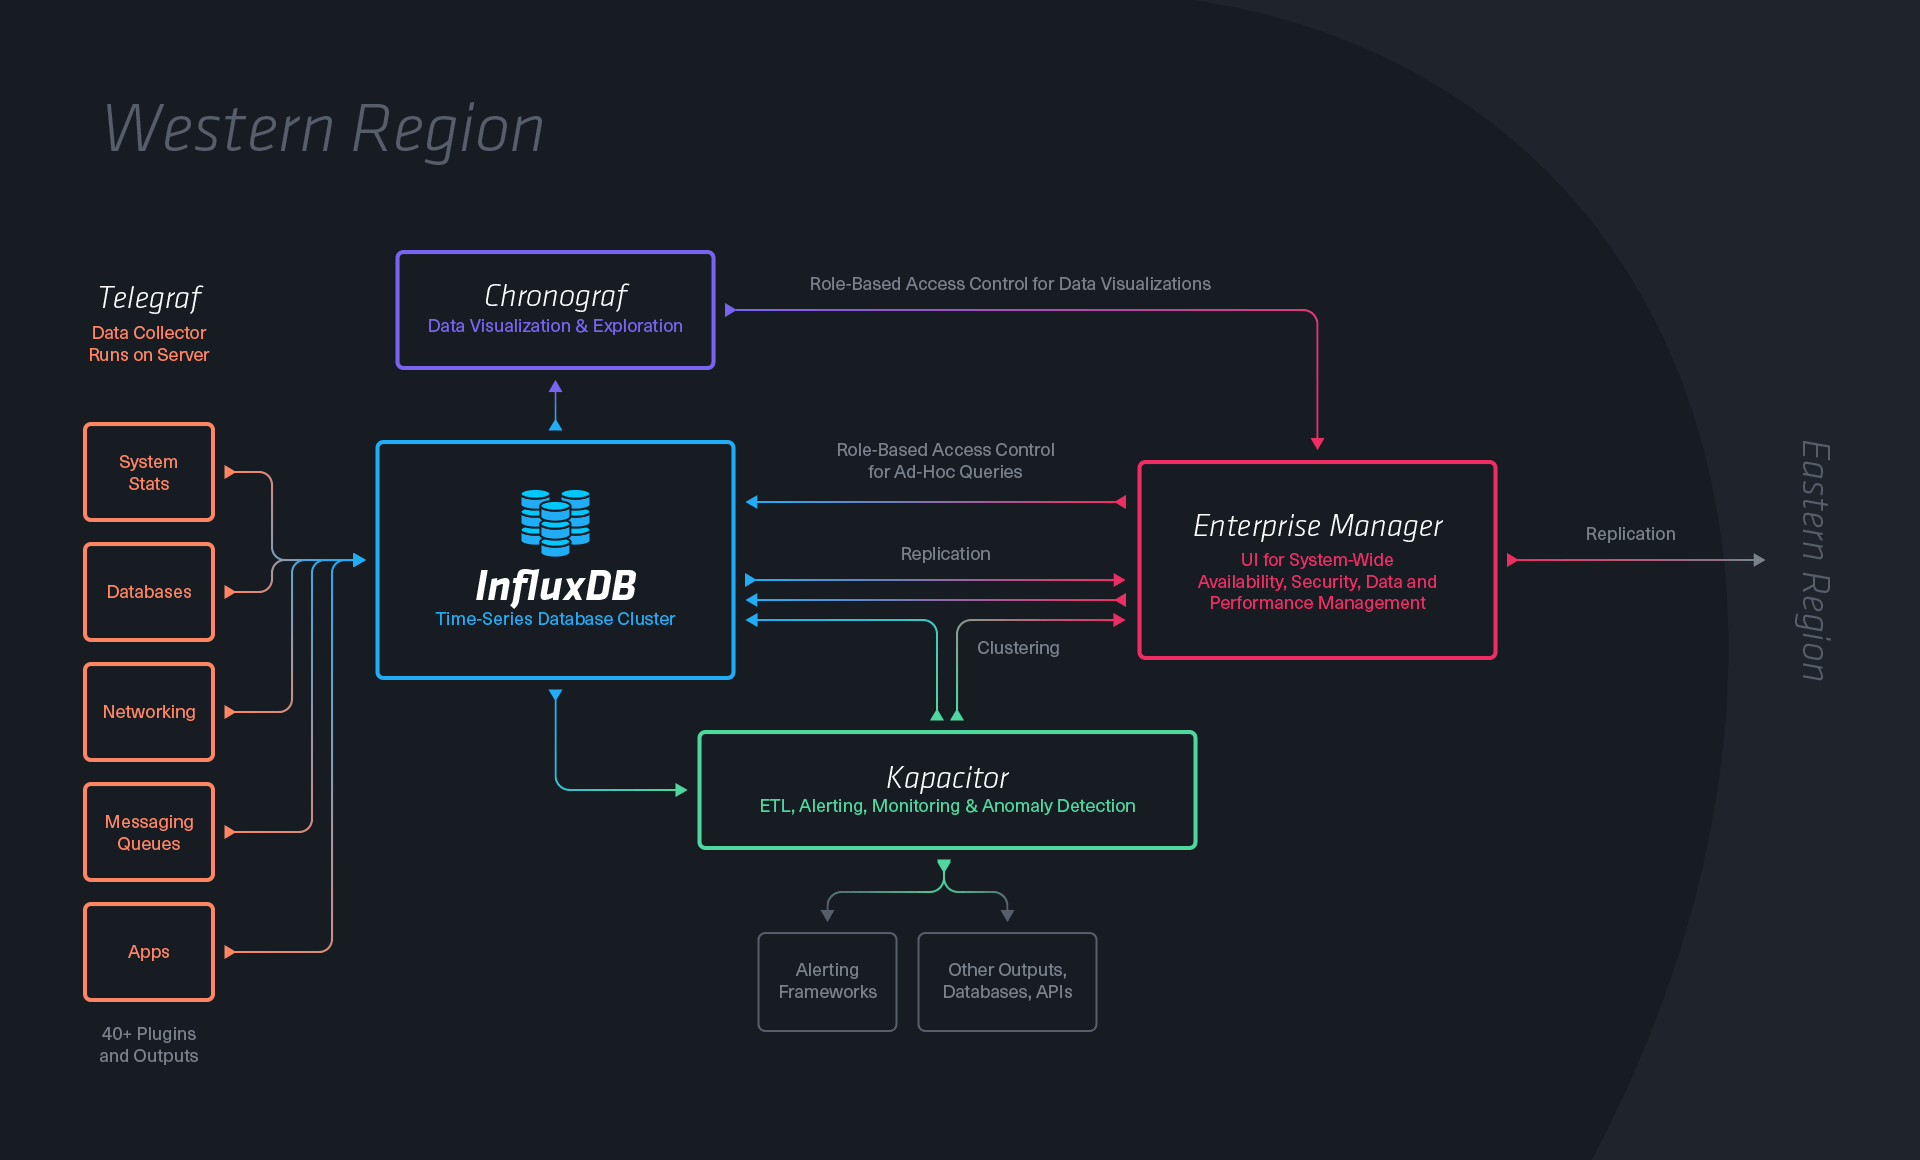
\includegraphics[width=.9\linewidth,page=1]{img/TICK-Stack.png}\\
	\fontsize{4pt}{7.2}\selectfont
	\textit{https://www.influxdata.com/time-series-platform/}
\end{frame}

\begin{frame}{\insertsection}
	\begin{itemize}
		\setlength\itemsep{1em}
		\item Unser Stack vielleicht als Mischung?
		\item Viele Metriken, Verbindungsdaten, Auslastung etc
		\item Viele Logdaten von Bro \& Honeypot
		\item Time-Series DB sinnvoll für Metriken
		\item Query-Mächtigkeit von ES sinnvoll für Korrelation komplexer (Log-) Text-Daten
	\end{itemize}
\end{frame}



%\section{Docker \& Rocket}
%\section{Kubernetes \& Mesosphere}


% Literatur
%\section{\bibname}
%\begin{frame}[allowframebreaks]{\bibname}
%	\AtBeginSection{}
%	\nocite{*}
%	\bibliographystyle{apacite}
%	\bibliography{bib}
%\end{frame}


\end{document}